\section{Selective Attention Memory (SAM) Network}

%\begin{figure}[!b]
%\begin{minipage}{0.43\textwidth}
%	\centering
%	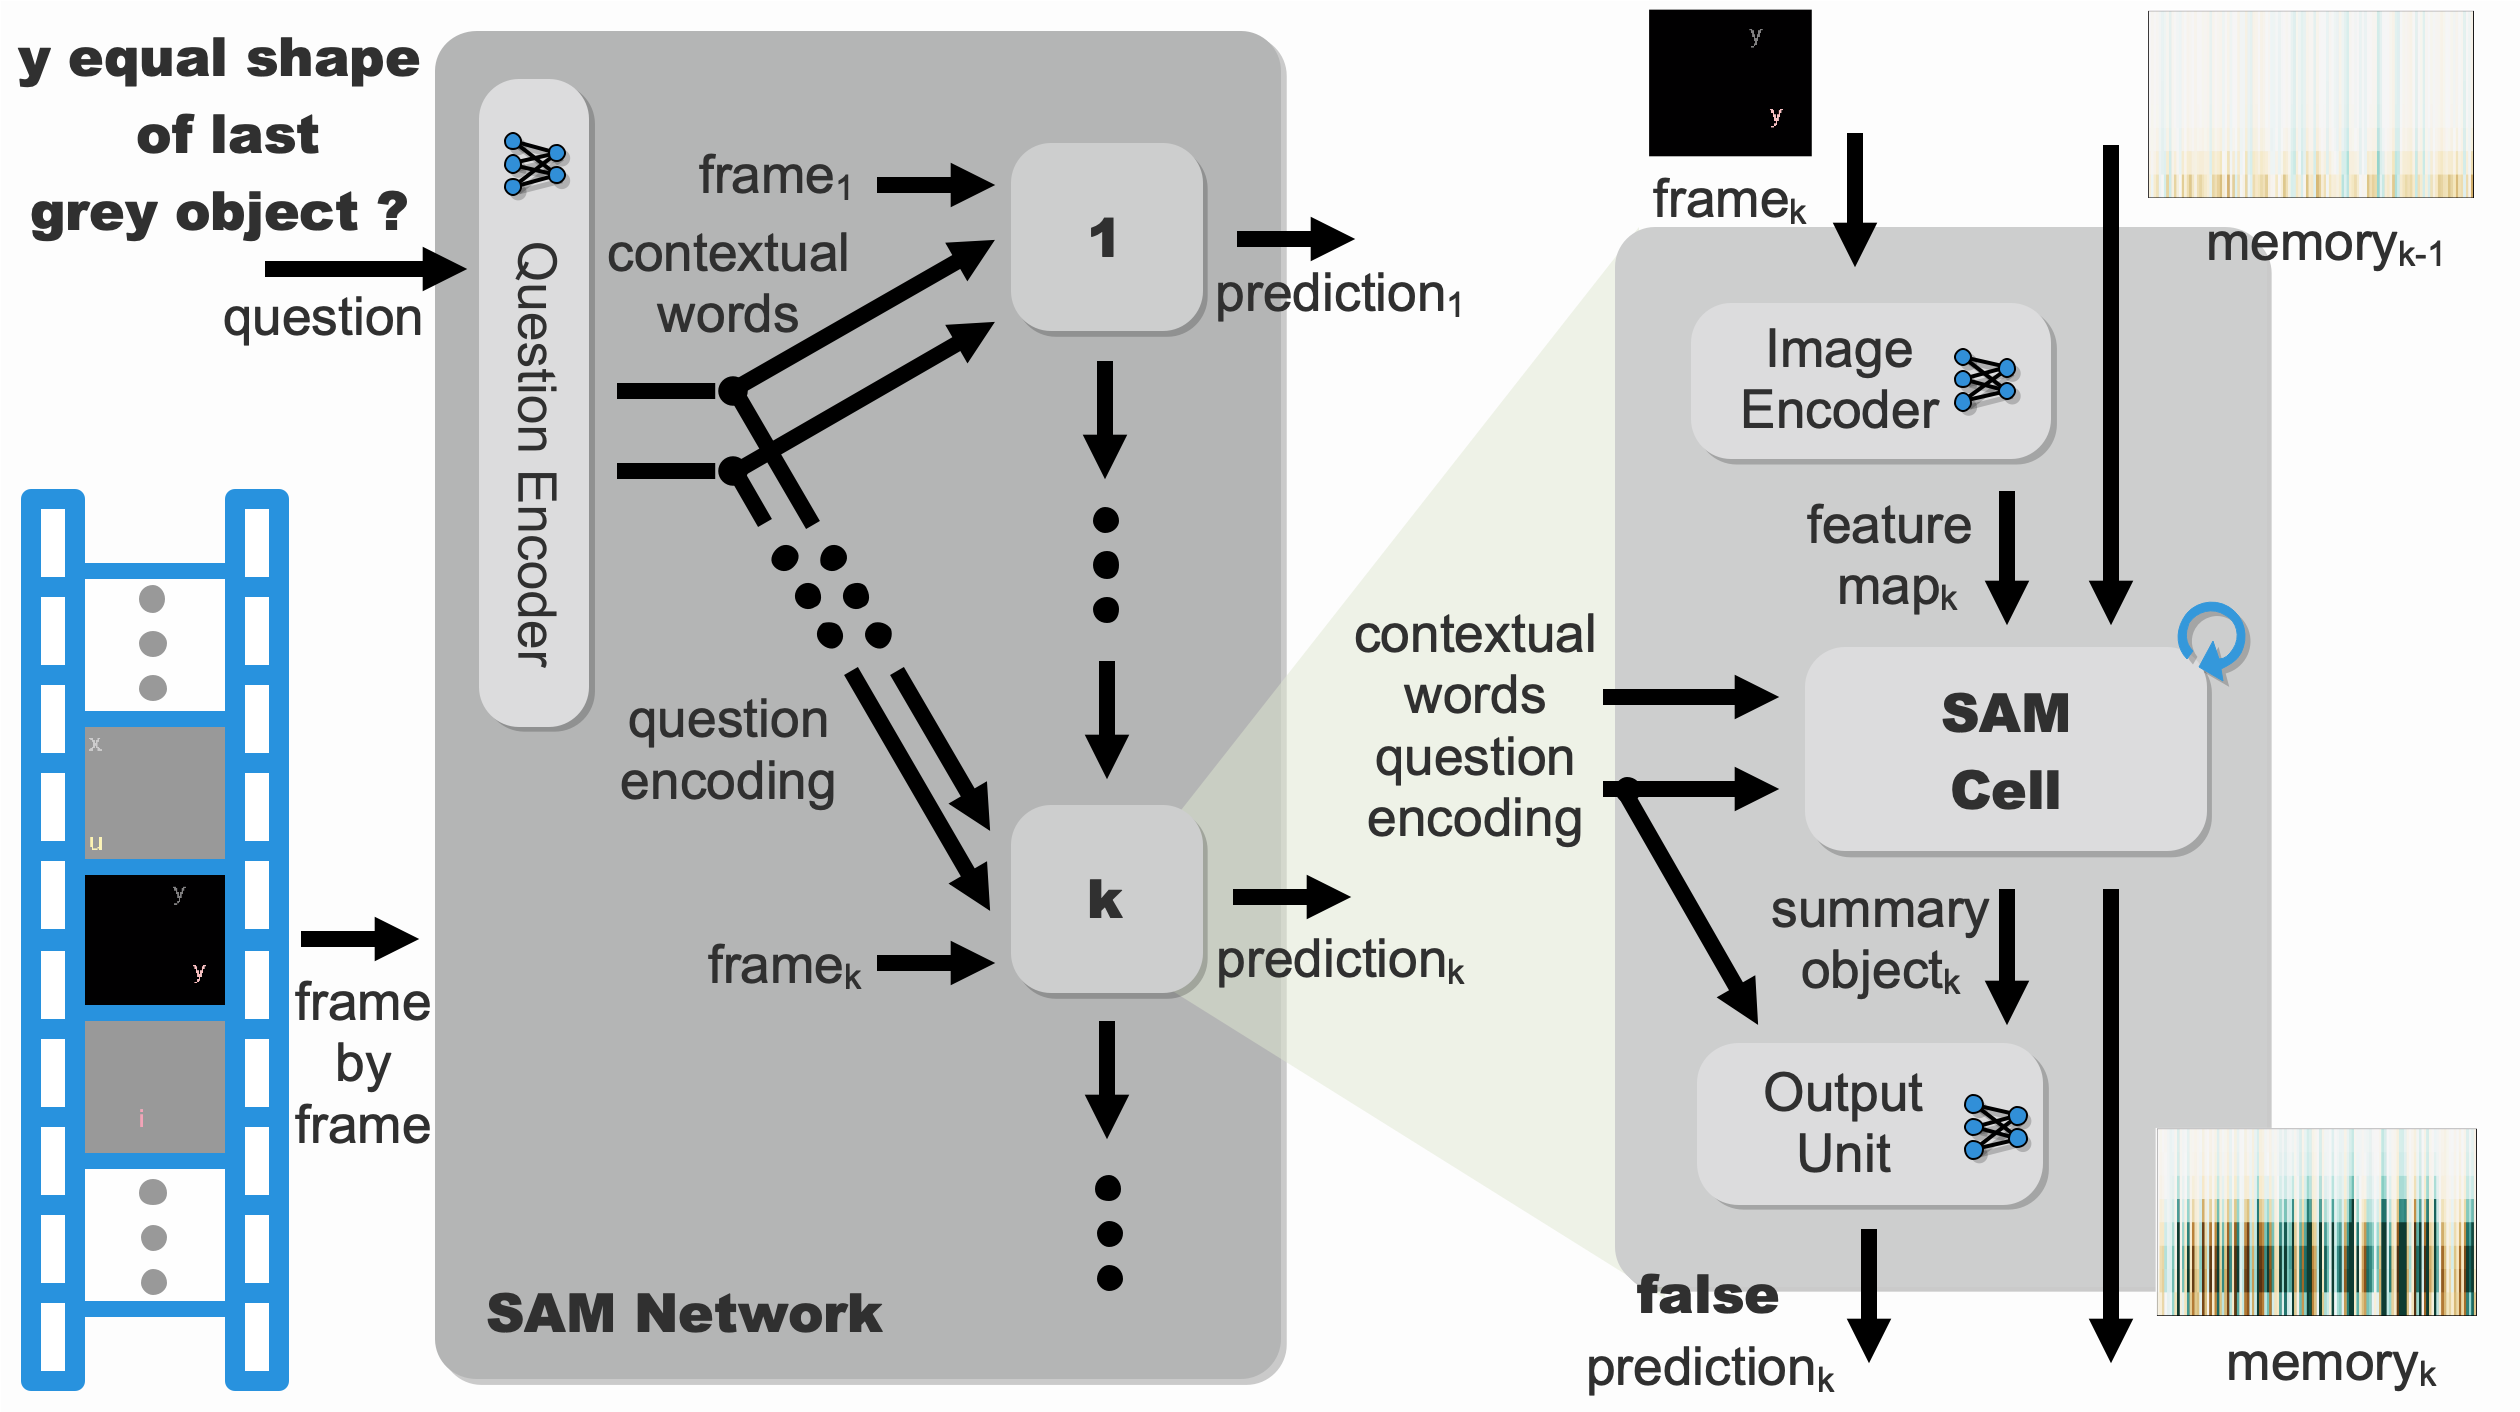
\includegraphics[width=\textwidth]{../img/architecture/samnet_architecture4}
%\end{minipage}\hfill
%\begin{minipage}{0.55\textwidth}
%	\centering
%	\includegraphics[width=\textwidth]{../img/architecture/samcell_reasoning}
%\end{minipage}\hfill
%\caption{General architecture of SAMNet (left) and a single reasoning step in SAMCell (right)}
%\label{fig:samnet}
%\end{figure}	

%Selective Attention Memory Network (SAMNet) is a end-to-end differentiable model made for video reasoning. It is a model based on attention mechanisms but also on a Selective Attention Memory which is able to store selected entities. This memory enables SAMNet to reason across multiple frames and perform spatio-temporal reasoning. 
%The core of SAMNet is based a recurrent cell called SAMCell. By aligning together a series of k SAMCells per frame, the network can perform k reasoning steps over a frame. At every new frame, a new series of k SAMCells is initiated. The SAMCell can read and write to memory at every frame using a content addressable mechanism. This section describes the model and the different units that composed a SAMCell. They are called the Question-driven Controller, the Visual Retrieval Unit, the Memory Retrieval Unit, the Reasoning unit, the Memory update unit, and the Summary Object Udpate Unit. 
%The model is also composed of an Image Encoder and a Question Encoder both responsible to pre-process the visual and textual inputs. The output unit is a classifier.
%All those modules are described below.
\ao{Method: Start high level, how different modules interface each other, and what the motivation is for each such a module. Then it should define standard parts such as attention over questions, and introduce all the variables that appear from nowhere. I would also like to see a more clear Figure 2 depicting the architecture. There is very little correspondence between that figure and the equations used in the paper.}

SAM Network (SAMNet for short) is an end-to-end differentiable recurrent model equipped with an external memory~(\cref{fig:samnet}). At the conceptual level, SAMNet draws from two core ideas:
iterative reasoning as proposed e.g. in MAC (Memory-Attention-Composition) Network~\cite{hudson2018compositional,marois2018transfer} and use of an external memory, as in Memory-Augmented Neural Networks such as NTM (Neural Turing Machine)~\cite{graves2014neural}, DNC (Differentiable Neural Computer)~\cite{graves2016hybrid} or DWM (Differentiable Working Memory)~\cite{jayram2018learning}.

A distinctive feature of the SAM Network is its frame-by-frame temporal processing approach, where a single frame can be accessed at once. This is a notable difference from~\cite{haurilet2019s}, which uses graph traversal reasoning. The recurrent nature of SAMNet does not prevent frame sequences longer than those used for training.
The memory locations store relevant objects representing contextual information about words in text and visual objects extracted from video. 
Each location of the memory stores a $d$-dimensional vector. %, where $d$ is a global parameter.
The memory can be accessed through either content-based addressing, via dot-product attention, or location-based addressing. Using gating mechanisms, correct objects can be retrieved in order to perform multi-step spatio-temporal reasoning over text and video.
A notable feature of this design is that the number of addresses $N$ can be changed between training and testing, to fit the data characteristics.

%\begin{figure}[t!]
%	\centering
%	\includegraphics[width=\textwidth]{img/architecture/samcell_reasoning}
%	\caption{Unfolded reasoning steps with operations performed by the SAMCell}
%	\label{fig:samcell}
%\end{figure}


SAMNet's core is a recurrent cell called the SAM Cell. Unrolling a new series of $T$ cells for each frame allows $T$ steps of iterative reasoning, similar to~\cite{hudson2018compositional}. Information flows between frames through the external memory. 
During the $t$-th reasoning step, for $t=1,2, \dots, T$, SAM Cell maintains the following information as part of its recurrent state:
(a) $\vec{c}_t \in \Reals^d$, the control state used to drive reasoning over objects in the frame and memory; and
(b) $\vec{so}_t  \in \Reals^d$, the summary visual object representing the relevant object for step $t$.
Let $\vec{M}_t \in  \Reals^{N \times d}$ denote the external memory with $N$ slots at the end of step $t$.
Let $\whead_t \in  \Reals^N$ denote an attention vector over the memory locations;
in a trained model, $\whead_t$ points to the location of the first empty slot in memory for adding new objects.

\begin{figure*}
	\centering
	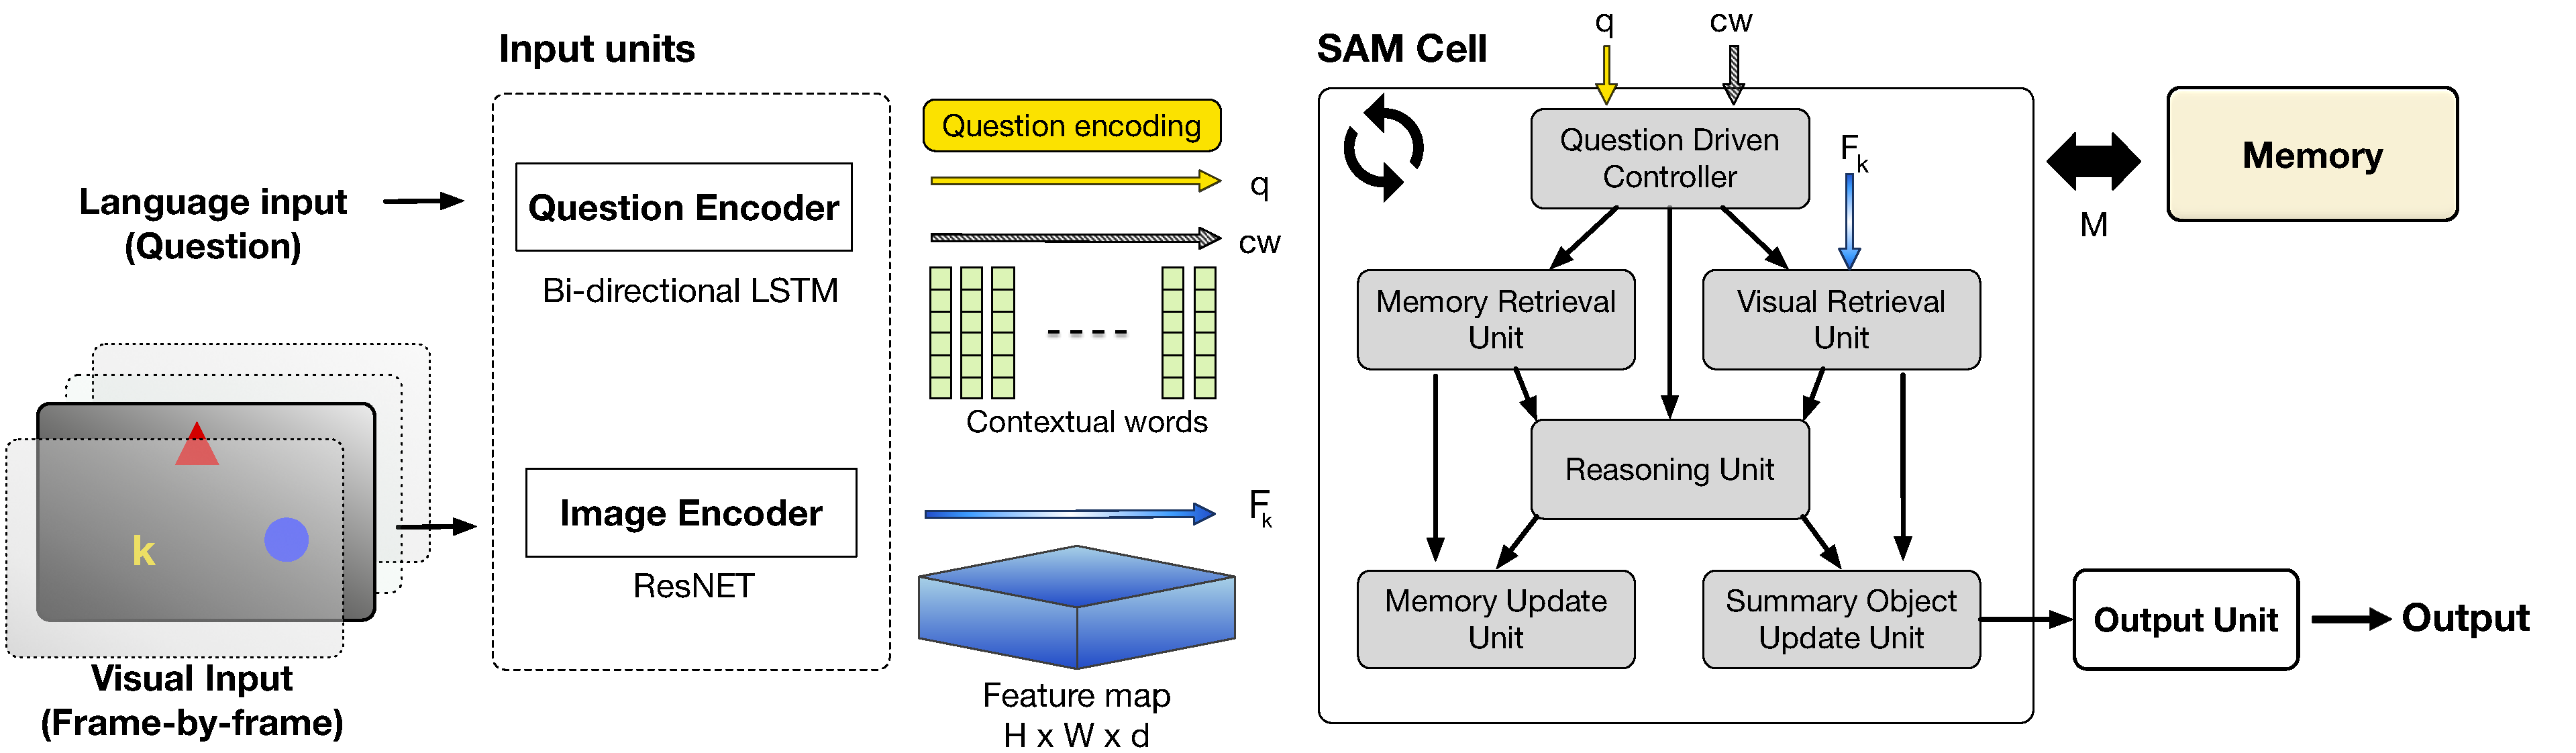
\includegraphics[width=\textwidth]{../img/architecture/SAMNETmodel}
	\caption{General architecture of SAMNet.}
	\label{fig:samnet}
\end{figure*}

\noindent{\textbf{Question-driven Controller.}}
This module drives attention over the question to produce $k$ control states, one per reasoning operation.
The control state $\vec{c}_t$ at step $t$ is then fed to a \emph{temporal classifier}, 
a two-layer feedforward network with ELU activation in the hidden layer of $d$ units.
The output $\bm{\tau}_t$ of the classifier is intended to represent the different temporal contexts (or lack thereof) associated with the word in focus for that reasoning step.	
For the COG dataset, we pick 4 classes to capture the terms labeled ``last'', ``latest'', ``now'', and ``none''.

The visual retrieval unit uses the information generated above to extract a relevant object $\vec{vo}_t$ from the frame.
A similar operation on memory yields the object $\vec{mo}_t$. The memory operation is based on attention mechanism, and resembles content-based addressing. Therefore, we obtain an attention vector over memory addresses that we interpret to be the \emph{read head}, denoted by $\rhead_t$.
%Note that the returned objects may be invalid, e.g., if the current reasoning step focuses on the phrase ``last red square'', $\vec{vo}_t$ is invalid even if the current frame contains a red square. 

\noindent{\textbf{Reasoning Unit.}}
%\paragraph{Reasoning Unit.}
This module is the backbone of SAMNet, which determines the gating operations to be performed on the external memory, as well as determining the correct object's location for reasoning.
To resolve whether we have a valid object from the frame (and similarly for memory), we execute the following reasoning procedure.
First, we compute a simple aggregate\footnote{%
	This is closely related to R\'{e}nyi entropy and Tsallis entropy of order~2.} of the visual attention vector $\vec{va}_t$ of dimension $L$ ($L$ denotes the number of feature vectors for the frame):
$vs_t = \sum_{i=1}^L [\vec{va}_t(i)]^2$. It can be shown that the more localized the attention
vector, the higher the aggregate value.
We perform a similar computation on the read head $\rhead_t$ over memory locations.
We input these two values, along with the temporal class weights $\bm{\tau}_t$, into a 3-layer feedforward classifier with hidden ELU units to extract 4 gating values (in $[0,1]$) for the current reasoning step:
(a) $\imatch_t$, which determines whether there is a valid visual object;
(b) $\mmatch_t$, which determines whether there is a valid memory object. 
(c) $\doreplace_t$, which determines whether the memory should be updated by replacing a previously stored object with a new one; and
(d) $\doadd_t$, which determines whether a new object should be added to memory.
We stress that the network has to learn via training how to correctly implement these behaviors.

\noindent{\textbf{Memory Update Unit.}}
The unit first determines the memory location where an object could be added:
\[ \vec{w}_t = \doreplace \cdot \rhead_t + \doadd \cdot \whead_{t-1} \]
Above, $\vec{w}_t$ denotes the pseudo-attention vector that represents the ``location'' where the memory update should happen.
$\vec{w}_t$ sums up to at most 1 and can be zero, indicating in this case there is no need adding a new object nor replacing an existing object.
We then update the memory accordingly as:
\[ \vec{M}_t = \vec{M}_{t-1} \odot (\vec{J} - \vec{w}_t  \otimes \mathbf{1}) + \vec{w}_t  \otimes \vec{vo}_t,\]
where $\vec{vo}_t$ denotes the object returned by the visual retrieval unit. 
Here $\vec{J}$ denotes the all ones matrix, $\odot$ denotes the Hadamard product and $\otimes$ denotes the Kronecker product. 
Note that the memory is unchanged in the case where $\vec{w}_t = 0$, i.e., $\vec{M}_t = \vec{M}_{t-1}$.
We finally update the write head so that it points to the succeeding address if an object was added to memory or otherwise stay the same.
Let $\whead'_{t-1}$ denote the circular shift to the right of $\whead_{t-1}$ which corresponds to the soft version of the head update.
Then:
\[ \whead_t = \doadd \cdot \whead'_{t-1} + (1-\doadd) \cdot \whead_{t-1} \]

\noindent{\textbf{Summary Update Unit.}}
%\paragraph{Summary Update Unit.}
This unit updates the (recurrent) summary object to equal the outcome of the $t$-th reasoning step.
We first determine whether the relevant object $\vec{ro}_t$ should be obtained from memory or the frame according to:
\[ \vec{ro}_t = \imatch_t \cdot \vec{vo}_t + \mmatch_t \cdot \vec{mo}_t \]
Note that $\vec{ro}_t$ is allowed to be a null object (i.e. 0 vector) in case neither of the gates evaluate to true.
Finally, $\vec{so}_t$ is the output of a linear layer whose inputs are $\vec{ro}_t$ and the previous summary object $\vec{so}_{t-1}$.
This serves to retain additional information in $\vec{so}_{t-1}$, e.g., if it held the partial result of a complex query with Boolean connectives.


%For details of the modules not covered here, please see the appendix.